\documentclass[english]{article}
\usepackage[T1]{fontenc}
\usepackage{natbib} % citations
\usepackage{csvsimple}
\usepackage{pgfplotstable}
\usepackage{rotating} % to rotate tables
%% tikz packages
\usepackage{tikz}
\usepackage{forest}
\usetikzlibrary{trees, arrows, shapes.geometric, positioning}
\usepackage{standalone}
%% text packages
\usepackage{siunitx} % fake ° symbol \ang{}
\usepackage[super]{nth} % for 1st, 2nd etc. \nth{}
\usepackage{hyperref}

\newcommand{\etoxbase}{Etox-Base}
\newcommand{\epa}{EPA ECOTOX data base}
\newcommand{\app}{http://139.14.20.252:3838/etox-base-shiny/}
\newcommand{\git}{https://github.com/andreasLD/etox-base}
\newcommand{\gitapp}{https://github.com/andreasLD/etox-base-shiny}
\newcommand{\ecfifty}{EC\textsubscript{50}}


\listfiles


\begin{document}


\title{Etox-Base: A tool to derive exposure endpoints from chemical test results}

\author{Andreas Scharm{\"u}ller\textsuperscript{1{*}},
        Verena Schreiner\textsuperscript{1},
        Ralf B. Sch{\"a}fer\textsuperscript{1}}

\maketitle
\thispagestyle{fancy}

1. Institute of Environmental Sciences, University of Koblenz-Landau Fortstraße 7, 76829 Landau, Germany {*}corresponding author(s):
Andreas Scharm{\"u}ller (scharmueller@uni-landau.de)

\begin{abstract}

<WRITE ABSTRACT>

\end{abstract}

\section*{Background \& Summary [max 700 words]}

A large number of chemicals such as pharmaceuticals, pesticides and synthetic hormones are in daily use all over the world with insufficient knowledge about possible adverse effects on the environment. In Europe alone some 100,000 chemicals are estimated to be in current use, whereof 30,000 are produced in quantities larger than one ton per year \citep{breithaupt_costs_2006}. Chemicals are brought to the environment deliberately - as it is the case of pesticides, or arrive therein as a byproduct from other processes (e.g. atmospheric emissions or wastewater) \citep{schwarzenbach_challenge_2006}. Ecosystems provide essential services to human societies such as drinking and irrigation water, food and climate regulation. These services are products of different ecosystem functions that crucially depend on the integrity of the populations and communities that drive these ecosystem functions. However, besides habitat degradation, climate change and nutrient enrichment, pollution with man-made chemical toxicants threatens these populations and communities in various ways which are currently not fully understood \citep{steffen_anthropocene_2007}. Pollution with man-made chemical toxicants was indeed identified as one of three major environmental problems for which research gaps hamper the derivation of planetary boundaries, i.e. thresholds beyond which irreversible state shifts may occur \citep{steffen_anthropocene_2007}. Bernhardt et al. \citet{bernhardt_synthetic_2017} argue further that the knowledge gap how chemicals effect populations and communities and hence ecosystem functions and ecosystem services, would also impede society’s ability to accomplish the Sustainable Development Goals of the United Nations. According to Breithaupt \citet{breithaupt_costs_2006} less than one percent of chemicals released to the environment are thoroughly tested. Although for some chemicals advanced and standardized \citep{oecd_oecd_2018} test methods have been developed, ecotoxicological tests for a lot of chemicals, especially newly emerging ones remain scarce and if existent, the information is represented sparsely and in inconsistent formats. \citep{gessner_fostering_2016}. Therefore we developed a data base that collects, processes and aggregates ecotoxicological tests results in order to subsequently publish it in an harmonized form as a web application - the \etoxbase tool: \href{http://139.14.20.252:3838/etox-base-shiny/}. This should facilitate researchers the access to ecotoxicological test results and support modern chemical risk assessment (CRA) workflows. The \etoxbase makes use of ecotoxicological test data, obtained from the ECOTOXicology knowledgebase (ECOTOX) created by the U.S. Environmental Protection Agency (EPA). ECOTOX collects raw, non harmonized ecotoxicological test data on on aquatic and terrestrial wildlife as well as plants and publishes it on a quarterly basis. By the time of writing it contained 926,108 test results, comprising 11,685 chemicals tested on 12,668 different species \citep{elonen_ecotoxicology_2018}. The collected ecotoxicological test data contain a variety of measured endpoints such as Effective Concentrations (\ecfifty{}) values, No-observed effect concentrations (NOEC) or lowest observed effect concentrations (LOEC). Likewise the data set contains different effect measures such as mortality, intoxication and growth as well as a multiplicity of test durations ranging from seconds to weeks or even years. The \etoxbase aggregates this information according to the user's inputs. These can then be used for the derivation of risk indicators such as Species Sensitivity Distributions (SSDs) \citep{posthuma_species_2002} and Toxic Units (TUs), which represent two prominent concepts to assess effects on organisms in ecotoxicology . The former combines toxicity data of several organism groups towards a chemicals to estimate effects on biotic communities, the latter refers to effects of a specific organism (group) towards a chemical. The two concepts are widely used in ecotoxicology \citep{kefford_definition_2011, schafer_effects_2011} since the allow for a comparison of toxicities across multiple chemicals and biological communities, respectively. Although performed on one and the same organism and chemical, outcomes of different ecotoxicological tests vary greatly due to differences in test parameters, genetic differences in individual populations or other irrepressible factors making a selection of appropriate test results for CRA laborious. The \etoxbase{} aims to relief this process and provide single toxicity values for organism, chemical and test duration combinations. The \etoxbase{} downloads every new version of the ECOTOX data base and performs several quality checks, e.g. unit harmonization, and cleaning steps on it. Hence, new scientific test results are constantly incorporated. Additionally the \etoxbase{} queries chemical- and organism-specific variables from other open data bases to fill information gaps such as water solubility, organism habitat or regional occurrence patterns in the ECOTOX data base.

\section*{Methods}

%%The Methods should include detailed text describing any steps or procedures 
%%used in producing the data, including full descriptions of the experimental 
%%design, data acquisition assays, and any computational processing (e.g. 
%%normalization, image feature extraction). Related methods should be grouped 
%%under corresponding subheadings where possible, and methods should be described 
%%in enough detail to allow other researchers to interpret and repeat, if required, 
%%the full study. Specific data outputs should be explicitly referenced via data 
%%citation (see Data Records and Data Citations, below). Authors should cite 
%%previous descriptions of the methods under use, but ideally the method 
%%descriptions should be complete enough for others to understand and reproduce 
%%the methods and processing steps without referring to associated publications. 
%%There is no limit to the length of the Methods section.

The \etoxbase{} consists of two parts of software: Firstly a processing pipeline (Fig. \ref{fig:pipeline}) downloads quarterly released new versions of the \epa{} and performs several preparation steps in R \citep{r_core_team_r_2017}, to then store the outcome in a PostgreSQL data base. This constitutes the basis upon which the R shiny web application is accessing the data \citep{r_core_team_r_2017}. The application itself is set of R functions that filter and aggregate the data according to a user's inputs \ref{fig:app}. Finally in the web application, a `filtered` and an `aggregated` data set as well as an interactive plot, for data exploration are returned. These two data sets can be downloaded. In the following these two parts are explained in detail, naming the respective R scripts in brackets.

\subsection*{Data acquisition \& preparation}

The EPA ECOTOX data is downloaded (bd\_epa\_download.R) and subsequently built into a PostgreSQL data base (bd\_epa\_postgres.R). Afterwards the data is imported into R for pre-processing (da\_epa1.R, da\_epa2.R, da\_epa3.R), which includes validity checks, removal of special characters, unit harmonizations and selection of relevant variables. Chemical abstract service (CAS) numbers, unique chemical identifiers together we taxon names are then used to query other data bases for additional information on chemicals and biota respectively. Chemical information is retrieved from the Compendium of Pesticide Common Names (qu\_aw.R) \citep{CITE_AW}, the Chemspider data base (qu\_chemspieder\_scrape.R) \citep{CITE-CHEMSPIDER}, from Eurostat <CITATION>, the Pubchem data base (qu\_pc.R) \citep{CITE_PUBCHEM}, and from the Physprop data base (qu\_pp.R) \citep{CITE_PHYSPROP}. These queries mostly rely on the webchem R-package \citep{szocs_webchem_2015-1}. For biota, habitat and occurrence information is queried from the World Register of Marine Species (WORMS) (qu\_worms2.R) \citep{WORMS} and from the Global Biodiversity Information Facility (GBIF) (qu\_rgbif.R) \citep{CITE_RGBIF} using the rgbif R-package \citep{chamberlain_rgbif_2018}. The acquired information is then merged (re\_merge.R) and information is combined (re\_combine.R). From there on the data set is analysed (re\_analyses.R) and checked (re\_checks\_internal.R) and finally compiled in one table (re\_final.R). This table is then used as the input for the filter and aggregation functions \ref{fig:pipeline}. For a detailed overview of what information is collected see table \ref{tab:scripts-pipeline}.

\begin{figure}
    \includestandalone[width=\textwidth, scale=0.1]{tikz/pipeline_organigram}
    \caption{Processing Pipeline}
    \label{fig:pipeline}
\end{figure}


\subsection*{The application}
The application is accessible through \app{} and was built in R, using the shiny web application framework \citep{chang_shiny_2018}. Users can define several input parameters \ref{tab:inputs} in the application's graphical user interface (GUI), handled in the ui.R script in order to adjust the aggregation according specific requirements. In doing so users execute R functions (fun\_filter.R, fun\_aggregation.R, fun\_filagg\_plot\_ly.R) loaded in the server.R script, which produce a 'filtered' and an 'aggregated' data set as well as an interactive overview plot. Only the 'aggregated' data set is presented in the GUI. However, both data sets can be downloaded via a download button.

\begin{figure}
    \includestandalone[scale=0.75]{tikz/application}
    \caption{Application}
    \label{fig:app}
\end{figure}

\subsection*{Aggregation}
The \etoxbase{} application aggregates the test results according to chosen filters in a two step process. Firstly the filtered test results are aggregated by the CAS number, the chosen taxon and the selected test duration. Secondly, the returned data is then aggregated by the CAS number. The former can't be influenced by the user and calculates either the minimum or the median depending on the amount of results to aggregate (n <= 2: minimum, if n > 2: median). Thereof the second step calculates the minimum, the maximum, the median, the geometric mean, or the arithmetic mean as an aggregate. 







\subsection*{Code availability}
%%For all studies using custom code in the generation or processing of datasets, 
%%a statement must be included here, indicating whether and how the code can be 
%%accessed, including any restrictions to access. This section should also include 
%%information on the versions of any software used, if relevant, and any specific 
%%variables or parameters used to generate, test, or process the current dataset. 

The processing code is stored in a Github reopsitory (\git{}). All processing scripts were written in R version 3.4.4. PostgreSQL 9.5 has been used to build the data base. Hence, R together with its packages \ref{tab:rpackages} and PostgreSQL suffice to rebuild the process. The code of the application itself is stored in a second Github repostitory (\gitapp{}). Since new versions of the EPA ECOTOX data base are published on a quarterly basis the data acquisition process is automated and new versions of the application are scheduled to be released regularly.

\begin{table}[h!]
    \centering
    \begin{tabular}{|l|l|l|l|}
        \hline
        Category        & Package       & Version   & Reference                     \\ \hline
        processing      & RCurl         & 1.95-4.11 & \citep{lang_rcurl_2018}       \\ \hline
        processing      & data.table    & 1.12.0    & \citep{dowle_data.table_2018} \\ \hline
        application     & shiny         & 1.1.0     & \citep{chang_shiny_2018}      \\ \hline
    \end{tabular}
    \caption{List of R packages used in compiling the data.\newline{}
    TODO: Automate version input and name generation - whole table\newline{}
    TODO2: debug chang\_shiny\_2018 reference}
    \label{tab:rpackages}
\end{table}



\section*{Data Records}
%%Please explain each data record associated with this work, including
%%the repository where this information is stored, and an overview of
%%the data files and their formats. Each external data record should
%%be listed in Data Citation section at the end of this template, and 
%%records should be cited throughout the manuscript as, for example 
%%(Data Citation 1). 
%%
%%Tables should be used to support the data records, and should clearly indicate 
%%the samples and subjects, their provenance, and the experimental manipulations 
%%performed on each. They should also specify the data output resulting from each 
%%data-collection or analytical step, should these form part of the archived record. 
%%Please see the submission guidelines at the \emph{Scientific Data} website, and 
%%our Word templates for more information on preparing such tables. 





\section*{Technical Validation}
%%This section presents any experiments or analyses that are needed
%%to support the technical quality of the dataset. This section may
%%be supported by up figures and tables, as needed. This is a required
%%section; authors must present information justifying the reliability
%%of their data.

<PUT COMPARISON WITH PPDB DATA HERE?>

\section*{Usage Notes}
%%Brief instructions that may help other researchers reuse these dataset.
%%This is an optional section, but strongly encouraged when helpful
%%to readers. This may include discussion of software packages that
%%are suitable for analyzing the assay data files, suggested downstream
%%processing steps (e.g. normalization, etc.), or tips for integrating
%%or comparing this with other datasets. If needed, authors are encouraged
%%to provide code, programs, or data processing workflows when they may help 
%%others analyse the data. We encourage authors to archive related code in 
%%a DOI-issuing archive when possible, but code may also be supplied as 
%%supplementary information files. 
%%
%%For studies involving privacy or safety controls on public access
%%to the data, this section should describe in detail these controls,
%%including how authors can apply to access the data, and what criteria
%%will be used to determine who may access the data, and any limitations
%%on data use.

The \etoxbase{} is designed to support CRA of ecotoxicologists. With an increased amount of available ecotoxicological test data, it becomes fundamental to provide and distribute such information in reasonable formats, meaning accessible for humans as well as machines. Currently CRA often relies on test results of a few, well tested standard organism, such as \textit{Daphnia magna}, \textit{Pimephales promelas}, \textit{Selenastrum capricornutum}, although researchers have conducted experiments on a much greater variety of organisms (e.g. the 926,108 test results collected in the EPA ECOTOX data base). In order to locate ecotoxicological test data, researchers can rely on individual test results reported in publications <CITE>, on compiled and published data sets \citep{malaj_organic_2014} or on data bases such as the Pesticide Property Data Base (PPDB) \citep{lewis_international_2016}. Each data source has its limitations though: Collecting toxicity information from individual publications is laborious and using already compiled data from publications or data bases is often limited to a specific groups of chemicals, such as pesticides, biozides etc. The \etoxbase{}, making use of the EPA ECOTOX data base, the largest publicly available collection of ecotoxicological test results, aims to facilitate the data retrieval process by providing adequate aggregates (\ecfifty{}, NOEC, LOEC) of the tests results. These are then used for the calculation of SSDs, TUs or other risk indicators. SSDs try to extrapolate effects of chemicals towards organisms from species to a community level by fitting a statistical distribution to toxicity test results on organisms of different trophic levels in order to derive concentrations at which a specific fraction of organisms are effected (often at 5\% - HC\textsubscript{5} \citep{posthuma_species_2002}. Figure \ref{fig:ssd-isoproturon} shows an example of a SSD and the derived HC\textsubscript{5} value (red dassed line) created for the herbicide Isoproturon. TUs are another indicator of effects of chemicals on organisms. They are calculated by dividing a measured concentration (c) by an \ecfifty{} value (cf. Equation \ref{eq:tu}).

\begin{equation}
    TU_i = \frac{c_i}{\ecfifty}
    \label{eq:tu}
\end{equation}

\begin{figure}[h!]
    \dentering
    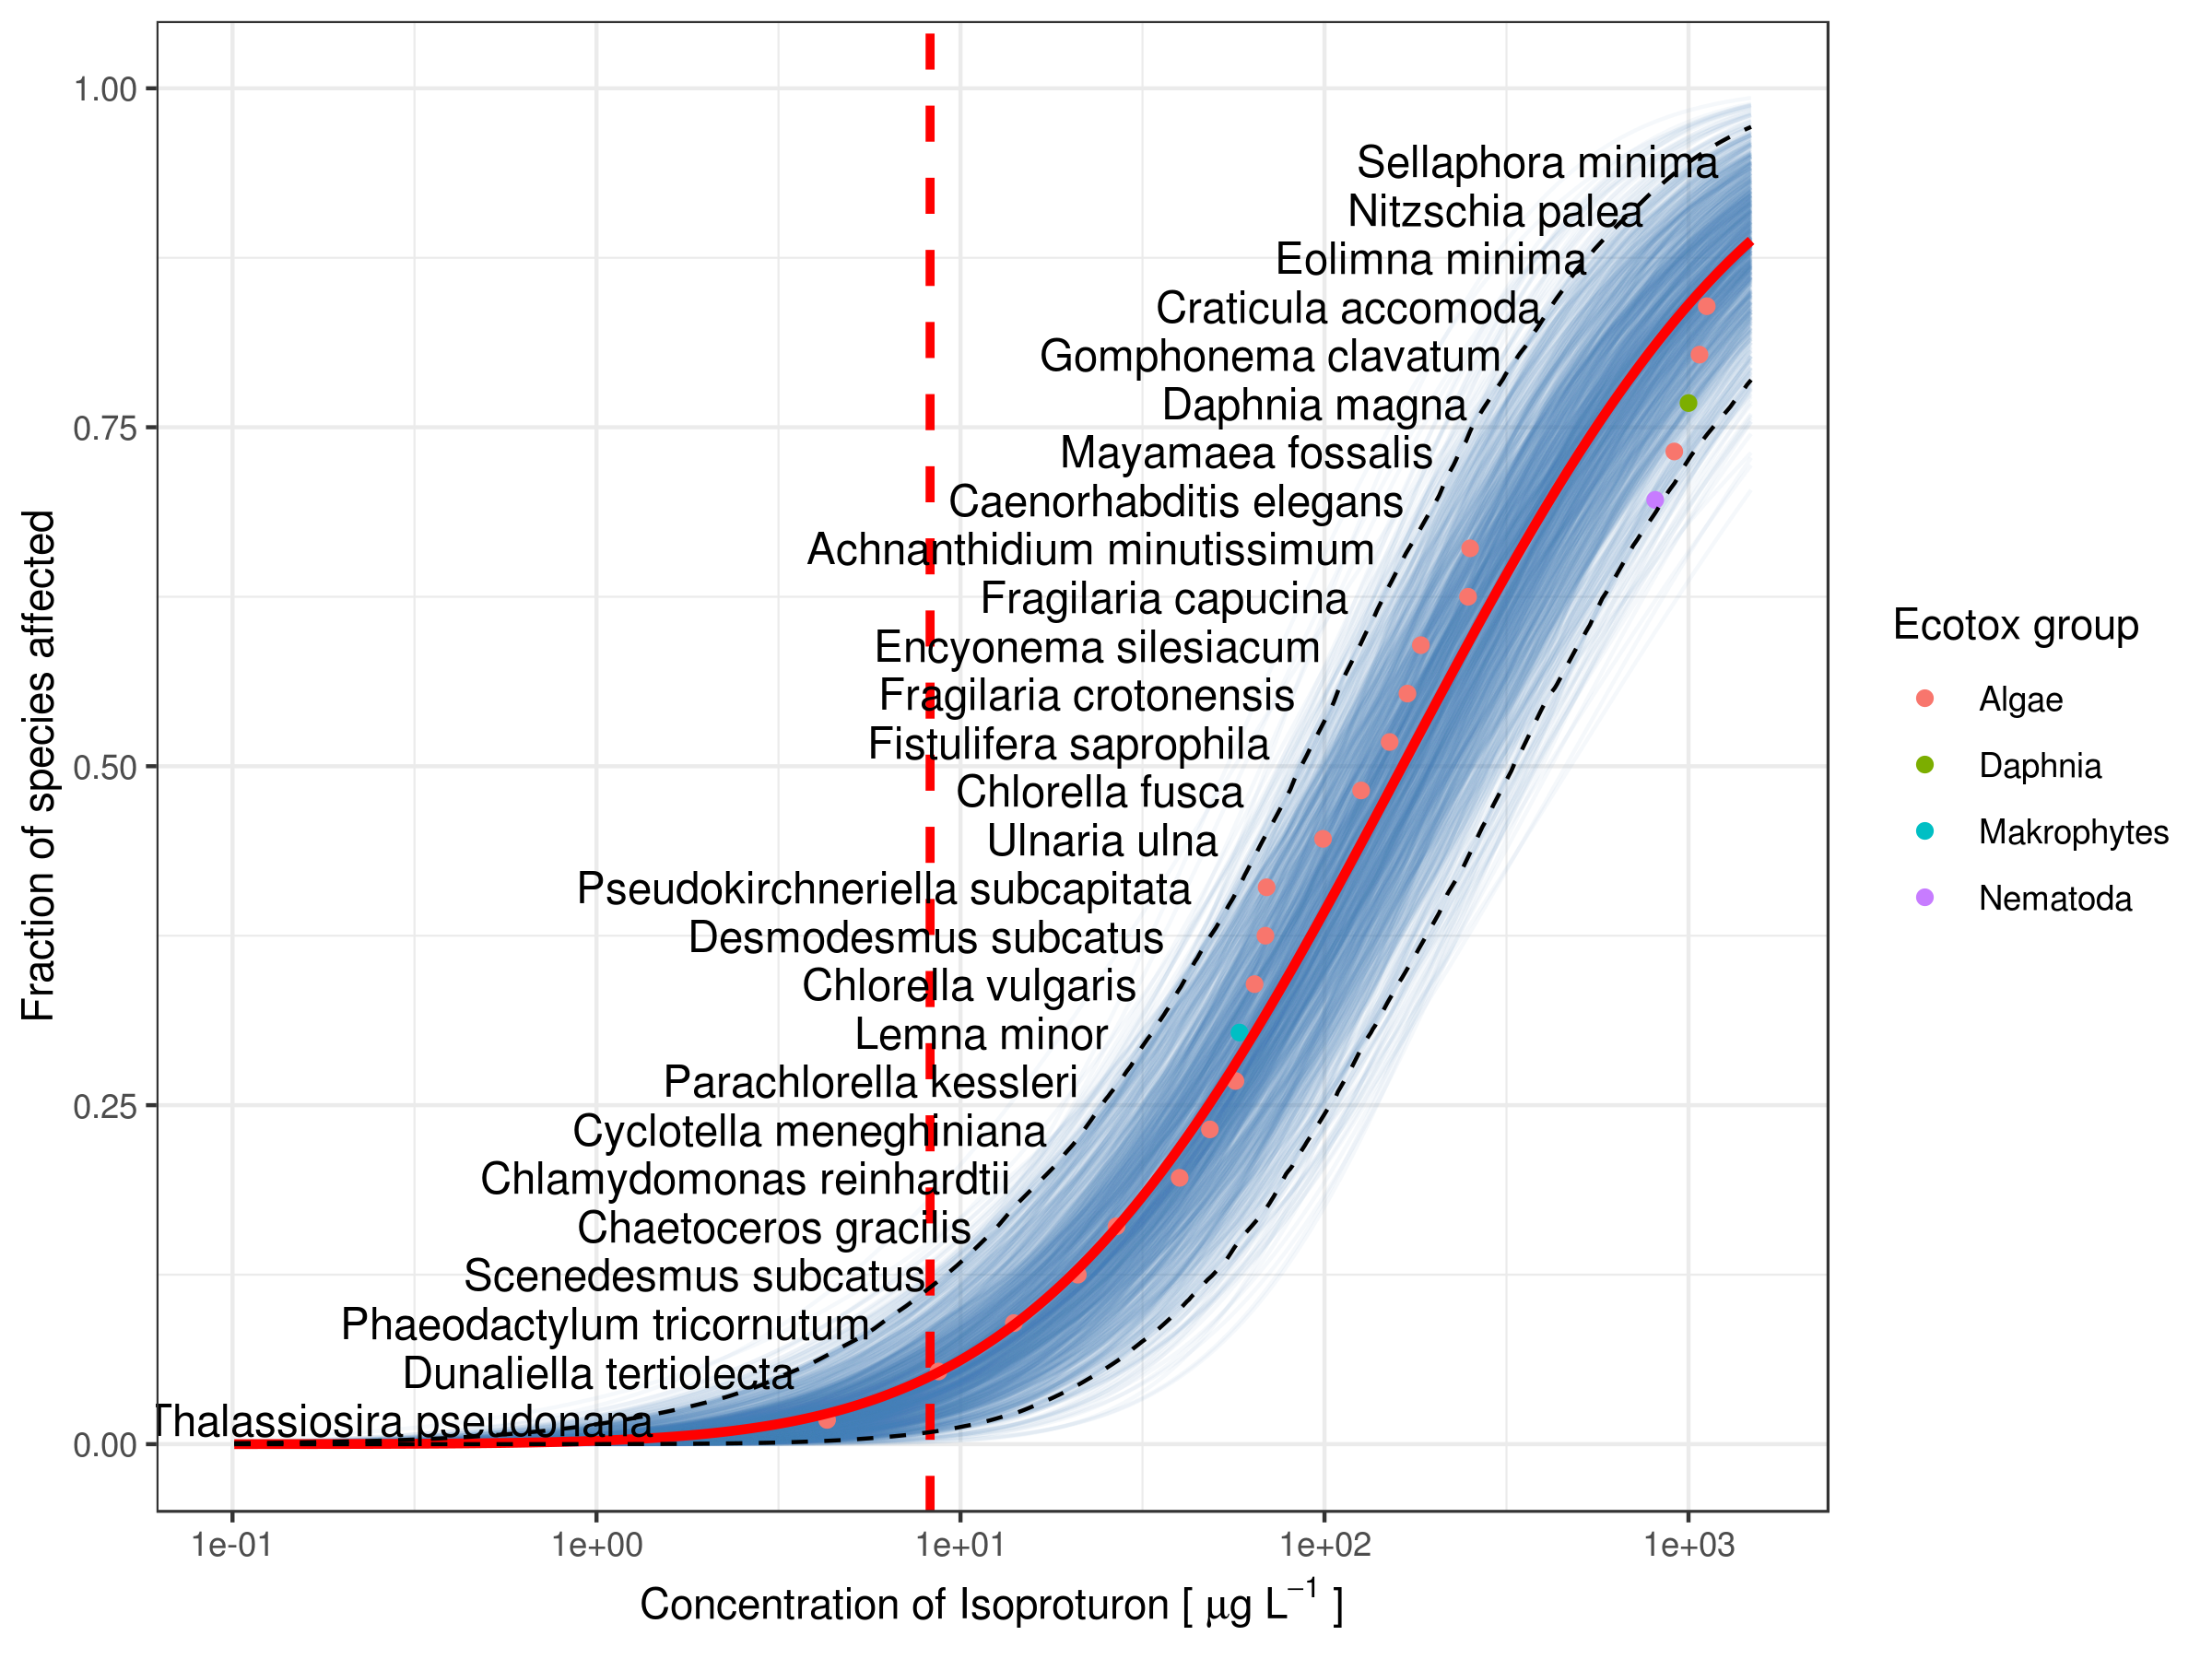
\includegraphics[width=1\linewidth]{article/figures/ssd2_boot.png}
    \caption{SSD plot showing the susceptibility of organisms towards the herbicide Isoproturon. The red line represents the fit and the red dashed line marks the HC\textsubscript{5} value, which is a common measure in CRA. The legend denotes common organism groups used in ecotoxicology.}
    \label{fig:ssd-isoproturon}
\end{figure}

\subsection*{Filter and Aggregate}

In the application's GUI, the user can choose among different parameters to filter and aggregate the test data accordingly \ref{tab:inputs}. Percentage values next to inputs show the proportion of the respective option (e.g. \textit{Active Ingredient - 43\%} indicates that 43\% of the data are Active Ingredients). The user can filter for compound-specific filters, including the CAS number, the concentration type (e.g. Active Ingredient, Formulation), the chemical class (e.g. Insecticides, Metals) and taxon-specific filters, including common taxonomic groups (e.g. Daphniidae, Algae), the organism habitat (e.g. freshwater) and the continent (e.g. Europe, Asia). Regarding the test parameters the user can choose test durations (in hours), Effect groups (e.g. Mortaliy, Population, Growth) and Endpoints (\ecfifty, EC\textsubscript{10}, LOEC or NOEC). Besides that, two cleaning steps can also be chosen. Firstly the application allows to exclude test results exhibiting concentrations that are higher than the actual water solubility of the respective chemical at \ang{20} C. Secondly the user can choose to exclude outliers (cf. Table \ref{tab:scripts-app}). The outliers are selected as values that exceed lower (0.25) and the upper (0.75) quartile by 1.5 times the inter-quartile range. As aggregates the user can choose the minimum, the maximum, the median, the geometric mean or the arithmetic mean. All the steps described in this section are selectable in the GUI and are executed at each click by the application. The drop down menu `Download data` allows to download a filtered data set as well as an aggregated data set.
The \etoxbase{} application can be accessed here: \app{}.


\begin{table}[h!]
\begin{tabular}{|l|l|l|l|}
\hline
Menu   & Group       & Subgroups              & Options \\ \hline
Filter      & Compound    & CAS                    & input CAS \\ \hline
Filter      & Compound    & Concentration type     & Active Ingredient; Formulation; Total \\ \hline
Filter      & Compound    & Chemical class         & Insecticides; Herbicides; Metals \\ \hline
Filter      & Taxon       & Taxon                  & Choose a taxon \\ \hline
Filter      & Taxon       & Organism habitat       & freshwater; terrestrial; marine; brackish \\ \hline
Filter      & Taxon       & Continent              & North America; Asia; Europe \\ \hline
Filter      & Test        & Duration               & enter duration in hours \\ \hline
Filter      & Test        & Effect groups          & MOR - Mortality; POP - Population \\ \hline
Filter      & Test        & Endpoins               & EC50, LOEC, LOEL \\ \hline
Filter      & Checks      & Water solubility check & yes/no \\ \hline
Filter      & Checks      & Remove outliers        & yes/no \\ \hline
Aggregation & Aggregation & Aggregate              & Minimum; Maximum; Median \\ \hline
\end{tabular}
\caption{\etoxbase GUI paramters to choose.}
\label{tab:inputs}
\end{table}



Generally it has to be stated here that the returned values are subject to change, as new tests will be constantly incorporated into the \etoxbase{}. However, we expect values of well tested chemical-organism combinations (i.e. high N <MAYBE PUT NUMBER HERE - CITATION>) to be relatively stable. Yet, returned values from the \etoxbase{} are certainly influenced by individual tests procedures and characteristics, such as pH, temperature or conductivity to just name a few. However, using the median or the geometric mean as an aggregate allows for an adequate estimation of the central tendency of the toxicity of a chemical towards an organism group. The geometric mean is recommended, as it is in comparison to the arithmetic mean considerably less influenced by outliers and is suitable for skewed data. Also, the geometric mean is preferable in contrast to the median, since the median completely ignores the influence of large or small values, making it unreliable for small data sets <CITATION GEOMETRIC MEAN>.

Other initiatives, with different, though partly overlapping aims accumulating existing ecotoxicological test data are published online. The PPDB provides validated ecotoxicological test results for pesticides, narrowing chemicals to this group \citep{lewis_international_2016}. The Network of reference laboratories, research centres and related organisations for monitoring of emerging environmental substances (NORMAN) focuses on assembling river basin specific pollutants\citep{von_der_ohe_new_2011}. The EnviroTox data base \href{https://envirotoxdatabase.org/} makes also use of the \epa{} data in order to derive Predicted no-effect concentrations (PNEC) \citep{health_and_environmental_sciences_institute_hesi_envirotox_2019}. In comparison to the \etoxbase, these examples partly rely on the same data, yet not aiming to derive \ecfifty, LOEC and NOEC from it automatically.






\subsection*{Limitations}

SSDs aim to extrapolate from species to the community level while not ignoring environmental variables (e.g. pH, temperature, etc.) which can effect the toxicity of a specific chemical greatly \citep{posthuma_species_2002}. For a large number of the \epa{} tests, environmental variables are not recorded (See \ref{table:meta-variables} for proportions of missing entries per variable). Hence to some extent the reported test results inherit uncertainty. In this context we also call for more emphasis on machine-readability when publishing ecotoxicological test results <CITATION ON AS OF HOW MANY DATA POINTS MACHINES ARE NEEDED>. A lot of important information is still confined in continuous text of articles and therefore not ascertainable for large scale analyses.














\section*{Acknowledgements}
%%Text acknowledging non-author contributors. Acknowledgements should
%%be brief, and should not include thanks to anonymous referees and
%%editors, or effusive comments. Grant or contribution numbers may be
%%acknowledged. Author contributions Please describe briefly the contributions
%%of each author to this work on a separate line. 
%%
%%AK did this and that. 
%%
%%BG did this and that and the other. 


\section*{Competing financial interests}
%%A competing financial interests statement is required for all accepted
%%papers published in \emph{Scientific Data}. If none exist simply write,
%%``The author(s) declare no competing financial interests''.


\section*{Figures Legends}
%%Figure should be referred to using a consistent numbering scheme through
%%the entire Data Descriptor. For initial submissions, authors may choose
%%to supply this document as a single PDF with embedded figures, but
%%separate figure image files must be provided for revisions and accepted
%%manuscripts. In most cases, a Data Descriptor should not contain more
%%than three figures, but more may be allowed when needed. We discourage
%%the inclusion of figures in the Supplementary Information \textendash{}
%%all key figures should be included here in the main Figure section. 
%%
%%Figure legends begin with a brief title sentence for the whole figure
%%and continue with a short description of what is shown in each panel,
%%as well as explaining any symbols used. Legend must total no more
%%than 350 words, and may contain literature references. 


\section*{Tables}
%%Tables supporting the Data Descriptor. These can provide summary information
%%(sample numbers, demographics, etc.), but they should generally not
%%be used to present primary data (i.e. measurements). Tables containing
%%primary data should be submitted to an appropriate data repository. 
%%
%%Tables may be provided within the \LaTeX{} document or as separate
%%files (tab-delimited text or Excel files). Legends, where needed,
%%should be included here. Generally, a Data Descriptor should have
%%fewer than ten Tables, but more may be allowed when needed. Tables
%%may be of any size, but only Tables which fit onto a single printed
%%page will be included in the PDF version of the article (up to a maximum
%%of three). 

%\begin{sidewaystable}
%    \csvautotabular[respect all]{data/meta.csv};
%    \caption{Meta variables table};
%    \label{table:meta-variables};
%\end{sidewaystable}


\begin{table}[h!]
\begin{tabular}{|l|l|}
\hline
Script                      & Description                                      \\ \hline
run\_build.R                 & runs all sub scripts                             \\ \hline
setup.R                     & sets up the environment                          \\ \hline
bd\_epa\_download.R         & download EPA Ecotox data base                    \\ \hline
bd\_epa\_postgres.R         & build EPA Ecotox data base locally               \\ \hline
da\_epa1.R                  & raw EPA Ecotox data export                       \\ \hline
da\_epa2.R                  & process EPA Ecotox data                          \\ \hline
da\_epa3.R                  & reduce EPA Ecotox data                           \\ \hline
qu\_aw.R                    & query Compendium of Pesticide Common Names       \\ \hline
qu\_chemspider\_scrape.R    & query Chemspider data base                       \\ \hline
qu\_eurostat\_chem\_class.R & query Eurostat data set                          \\ \hline
qu\_pc.R                    & query PubChem data base                          \\ \hline
qu\_pp.R                    & query Physprop data base                         \\ \hline
qu\_worms2.R                & query WORMS data base                            \\ \hline
qu\_gbif.R                  & query GBIF data base                             \\ \hline
re\_merge.R                 & merge all data                                   \\ \hline
re\_combine.R               & combine information                              \\ \hline
re\_analyses.R              & ???                                              \\ \hline
re\_checks\_internal.R      & ???                                              \\ \hline
re\_final.R                 & create and write final table                     \\ \hline
wr\_dbase.R                 & write final table to data base                   \\ \hline
wr\_app.R                   & write final table and variables to app directory \\ \hline
wr\_meta.R                  & ???                                              \\ \hline
wr\_stats.R                 & ???                                              \\ \hline
\end{tabular}
\caption{Scripts that are used to process the data}
\label{tab:scripts-pipeline}
\end{table}

\begin{table}[h!]
\begin{tabular}{|l|l|}
\hline
Script                     & Description                                               \\ \hline
setup.R                    & sets up the environment                                   \\ \hline
ui.R                       & creates the graphical user interface of the application   \\ \hline
server.R                   & handles functions and data input and output               \\ \hline
fun\_filter.R              & function that filters the data                            \\ \hline
fun\_aggregation.R         & function that performs the aggregation                    \\ \hline
fun\_filagg\_plot\_ly.R    & creates interactive plot                                  \\ \hline
\end{tabular}
\caption{Scripts that used for the web application}
\label{tab:scripts-app}
\end{table}


\section*{Figure Legends}

\bibliographystyle{apalike}
\bibliography{refs/references-etox-base.bib,refs/references-etox-base-rpackages.bib,refs/references-etox-base-rshinypackages.bib}
% multiple refs have to be written w/o space

\section*{Data Citations}

\pagebreak
\section*{TODO}

\begin{itemize}

\item compare Etox-BAse output with PPDB

\item plot example SSD and TU

\item acute vs chronic

\item OECD guidlines are not machine readable

\item discuss flaws in column types (e.g some concentration entries contain '+' or '~' and are therefore not convertable to numeric) - This hampers large scale analysis greatly!

\pagebreak
\section*{MISC}

\begin{figure}
    \includestandalone[scale=0.5]{tikz/tree_source}
    \caption{Alternative processing pipeline}
    \label{fig:pipeline-tree}
\end{figure}

\section*{not included citations}
Put in citation \citep{hartung_chemical_2009} ? which claims that REACH won't meet their assumptions and say 54 million vertebrate animals are needed for tests that would cost €9.5 billion over the next ten years. I.e 20 times more animals, 6 times the costs in comparison to the official estimates 


\end{itemize}


\end{document}







